% Name your report <group>-<unique-name>.tex, (e.g., sls-jupiter.tex)
% to avoid name collisions.  For \label{} entries within a file,
% please use \<group>-<unique-name>-<your label} (e.g.,
% \label{sls-jupiter-figure}), again to avoid name collisions.  There
% is no need to use unique names with \cite{} since each report has
% its own citation namespace.

% You can also use \formattitle{Title}{Authors} to gain formatting
% control (e.g., footnotes on author names or controlling line breaks
% with \\) and \formatcontents{Title}{Authors}.  Since we did not need
% such control, we simply used \formattitlecontents{Title}{Authors}
% here.  Please do not put any special formatting in
% \formattitlecontents or \formatcontents as this will disturb the
% table of contents.

\formattitlecontents 
{Linear Analysis and Optimization of Stream Programs}
{Andrew Lamb, Bill Thies, Saman Amarasinghe}


% Please use the following \formatsection entries unless they are
% inappropriate: Introduction, Approach, Progress, Future, Research
% Support.
%
% Do not put a blank line after a \formatsection, as this affects the
% formatting.

\formatsection{Introduction}
More than fifty percent of the code that runs the Digital Signal Processors
(DSPs) in a modern cell phone is written in assembly language and the 
rest is written in annotated C\cite{gass-talk}. Clearly even the best 
compilers that DSP companies can produce are utterly failing to produce
optimizion necessary for programs that will run on the next generation
of signal processors.

The sheer volume of analysis required to make optimal use of the special 
purpose instructions in DSPs leaves compilers for standard languages such 
as C unable to perform many of the standard optimizations known to electrical 
engineers. Using StreamIt~\cite{streamit-asplos,streamitcc}, a domain-specific 
stream processing language, we have been exploring novel high-level automatic 
DSP optimizations that are intractable in a general-purpose
language.

\formatsection{Approach}
Our analysis and optimizations focus on filters which compute {\it linear} 
functions of their inputs. A filter computes a linear function if its
the computation it does to convert input to output can be described by a 
matrix operation. Many fundamental DSP operations such as filtering, the
Discrete Fourier Transform (DFT), upsampling and downsampling, can be described 
as linear functions. We have developed and implemented a simple dataflow 
algorithm that can determine which filters in a StreamIt program compute 
linear functions and the specific matrices which describe that computation.
Figure~\ref{fig:overview} (top) shows a filter, and Figure~\ref{fig:overview}
(bottom) shows how a matrix and a vector can be used to describe the same
computation.

\begin{figure}
\center
\begin{tabular}{cc}
  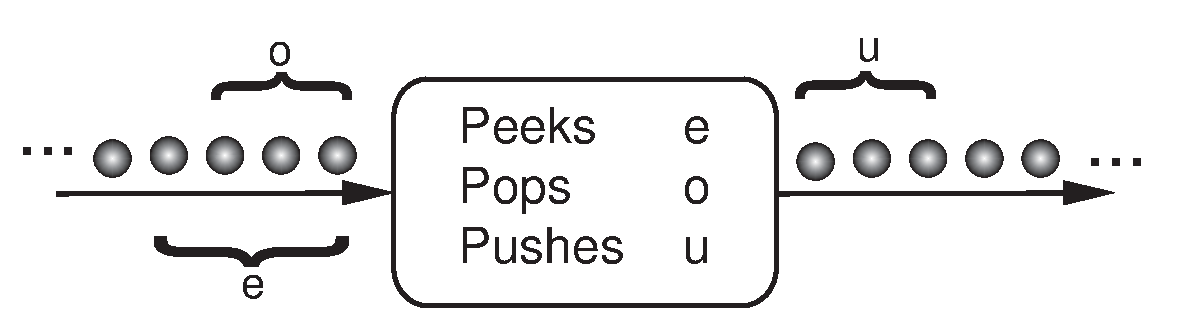
\includegraphics[height=1in]{cag-commit-streamit-linear-filter.eps} &
  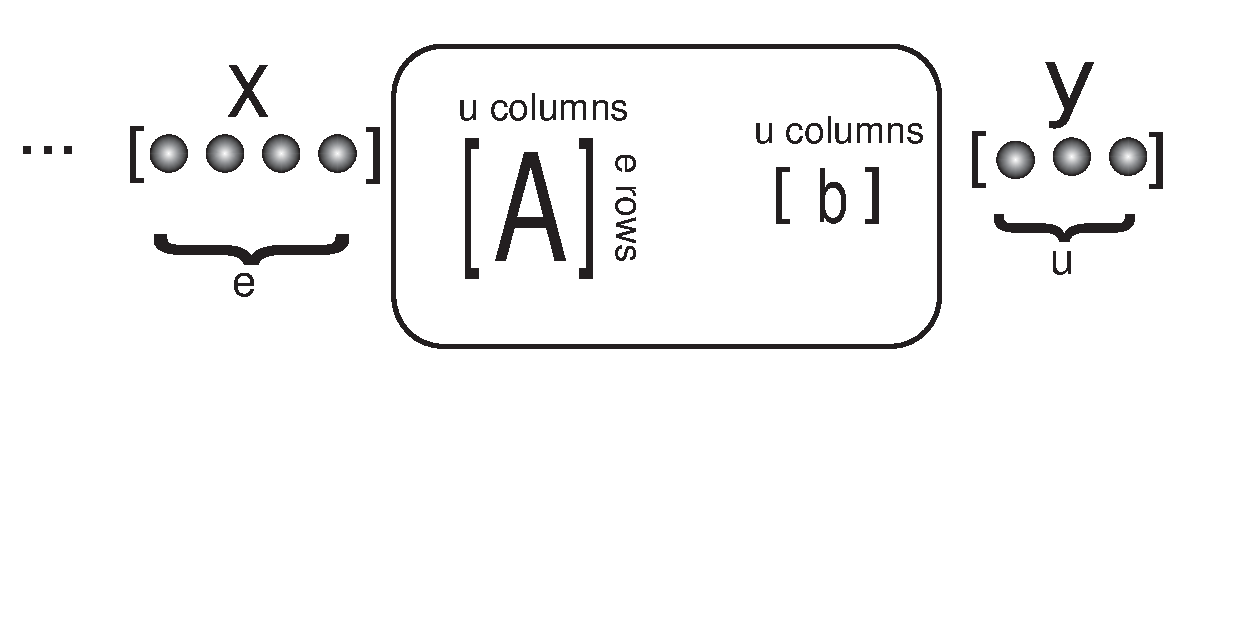
\includegraphics[height=1in]{cag-commit-streamit-linear-matrix.eps} \\
\end{tabular}
\caption{
  Top: StreamIt filter with I/O rates. 
  Bottom: Linear filter as a vector-matrix operation.
}
\label{fig:overview}
\end{figure}

A primary benefit of linear filter analysis is that neighboring
filters can be collapsed into a single matrix representation if both
of the filters are linear.  This transformation automatically
eliminates redundant computations in linear sections of the stream
graph, thereby allowing the programmer to write simple, modular
filters and leaving the combination to the compiler.  We have 
developed algorithms for a {\it linear expansion} operation that serves as a
building block for the combination techniques, collapsing {\tt pipeline}s 
and {\tt splitjoin}s into linear nodes.

To take advantage of our linear analysis framework, our compiler currently 
has two linear analysis optimizations. The first, {\it linear replacement}, 
replaces the largest possible linear sections of the program with filters 
that directly compute the calculation specified by the corresponding 
matrix representation. The second optimization, {\it frequency replacement}, 
replaces all streams which implement a sufficiently long convolution sum
using a standard frequency domain conversion.


\formatsection{Progress}
We have developed a fully automatic implementation of the linear analysis 
and optimizations as passes in the StreamIt compiler. Our preliminary results
are very promising. In our suite of benchmark applications, our optimizations
increased execution speed by an average factor of five, $6.5$ in the best 
case. Figure~\ref{fig:cag-commit-streamit-linear-speedup} (left) shows
the execution time increase for our benchmarks. The source of these impressive
speedups is shown in Figure~\ref{fig:cag-commit-streamit-linear-speedup}
(right). Both optimizations significantly reduce the number of floating point multiplications
in the benchmarks. 

XXXXXXXXXX

\begin{figure}
  \center
  \begin{tabular}{cc}
    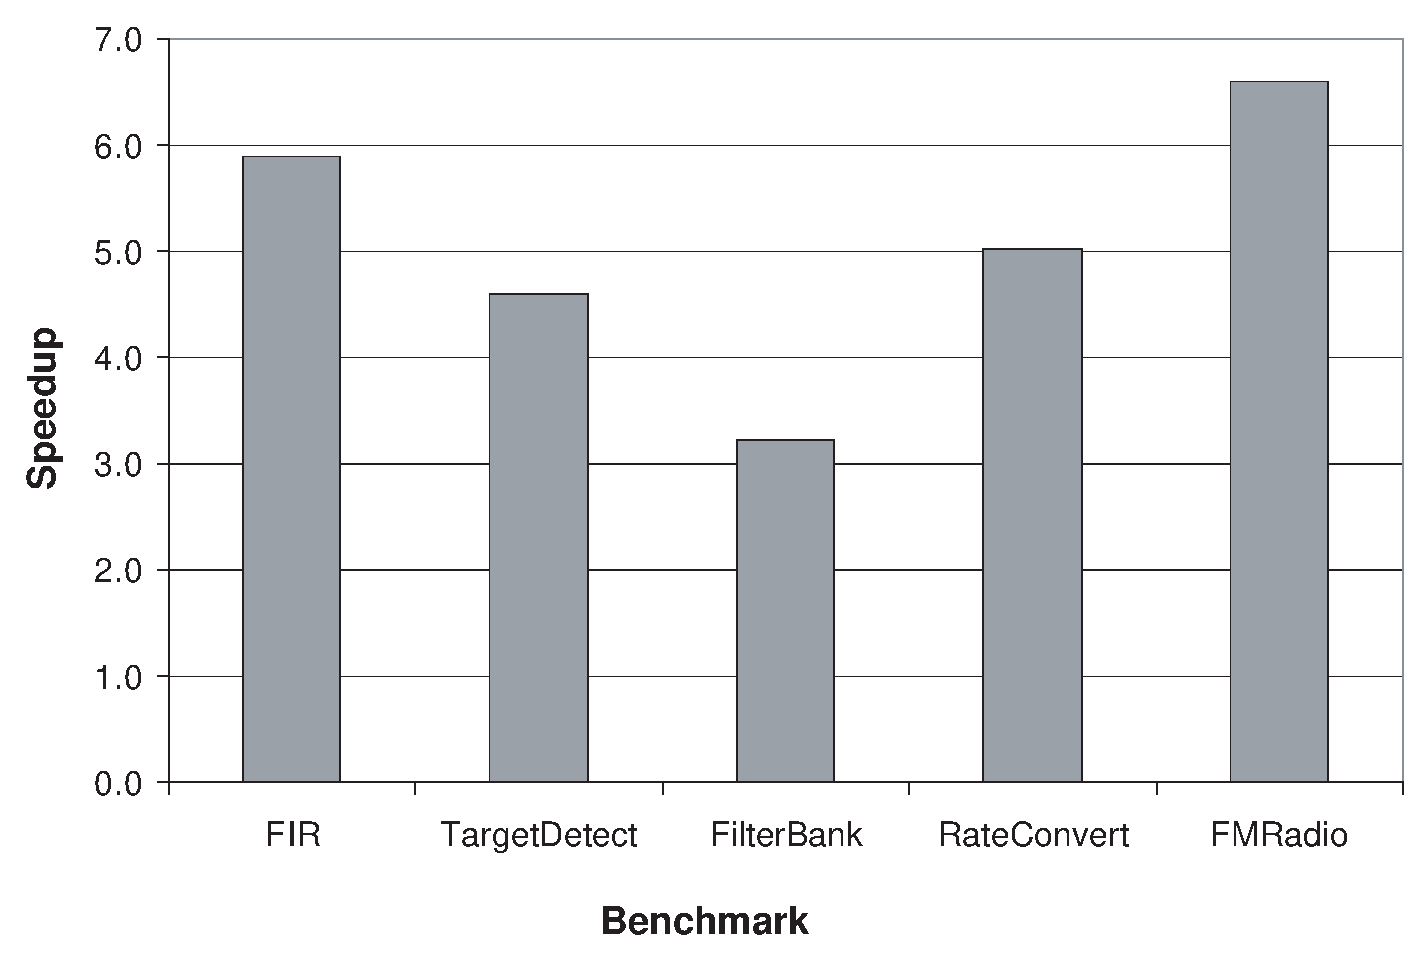
\includegraphics[height=2in]{cag-commit-streamit-linear-speedup.eps} &
    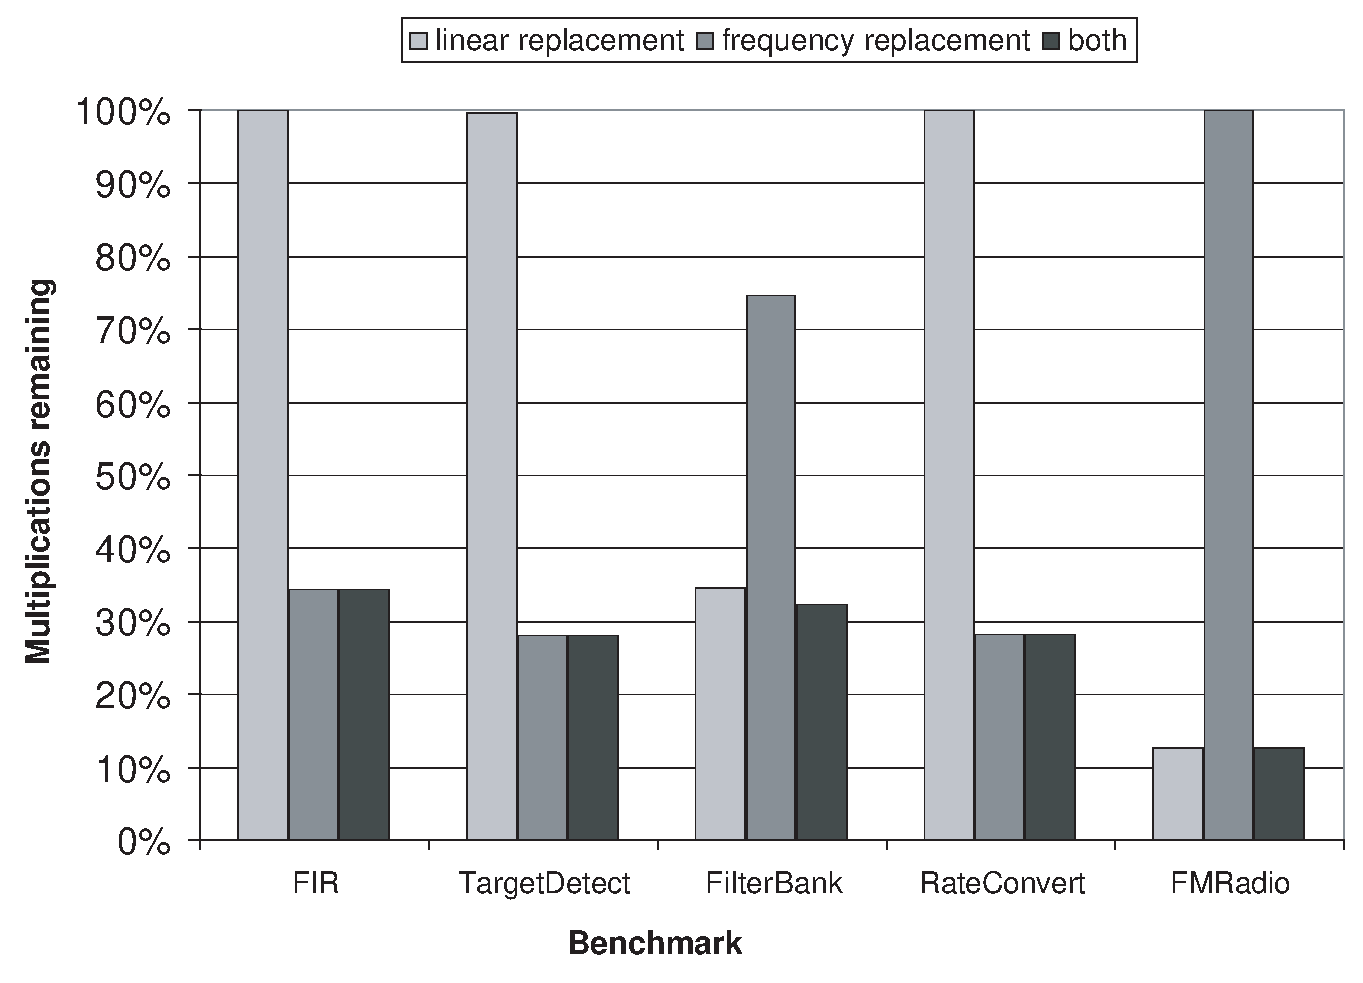
\includegraphics[height=2in]{cag-commit-streamit-linear-mults.eps} \\
  \end{tabular}
  \caption{
    Left: Execution speedup for each of the benchmarks with both linear 
    replacement and frequency replacement optimizations.
    Right: Percent of multiplication operations remaining after performing 
    linear replacement, frequency replacement, and both.
  }
  \label{fig:cag-commit-streamit-linear-speedup}
\end{figure}




\formatsection{Future}
For future research, we are developing new optimizations which make use
of our Linear Analysis framework. For instance, we are investigating saving
redundant partial results between filter executions in order to improve 
program performace. This optimization is very much like standard common
sub-expression eliminiation except that our optimization will remove common
subexpressions that occur in subsequenct calls to the same function.

Our current Linear Analysis framework requires that the only state
filters are allowed to use is the input tape. However, recognizing state
variables that are linear combinations of the input and previous state 
variables would allow us to analyze many other classes of programs. This
type of linear state is common in adaptive filters and in control 
applications.

Another area of potential research is in working with symbolic arrays. 
Currently, our analysis can only extract arrays with constant valued
entries. However, some applications actually perform linear operations
at runtime, but the values of the corresponding matrix are not compile
time constants. We can extend our framework to allow this sort of filter.
This type of analysis would allow, for instance, an FIR filter whose 
coefficients changed at runtime but at infrequent intervals. With an
updated framework we could still do the frequency transformation, and
we would know the approprate ways to updated the frequency coefficients
at runtime.

Additionally, we are planning on using the linearity information our
analysis extracts to make more informed decisions in other parts of the compiler.
For instance,  the StreamIt compiler is going to be extended to target 
a DSP architecture and we can make use of the linear information to 
take advantage of the specialized instructions that DSPs offer.


\formatsection{Research Support}
From DARPA and the Oxygen alliance (I don't know the details.....XXXXXXXXXXXXXXXXXXXX)
% Although the use of BibTeX is highly recommended, you can manually
% format your references as follows:
%
% \begin{thebibliography}{1}
%
% \bibitem{Zue00}
% V.~Zue, S.~Seneff, J.~R. Glass, J.~Polifroni, C.~Pao, T.~J. Hazen, and
% L.~Hetherington, ``\textsc{Jupiter}: A telephone-based conversational
% interface for weather information,'' \textit{IEEE Transactions on
% Speech and Audio Processing}, vol. 8, no.  1, pp. 85--96, Jan. 2000.
% 
% \end{thebibliography}

\bibtex{cag-commit-streamit-linear}
